\documentclass[12pt]{article}
\usepackage[utf8]{inputenc}
\usepackage{graphicx} % Required for inserting images
\usepackage[a4paper, margin=1in]{geometry} % Custom margins
\usepackage{fancyhdr} % For headers and footers
\usepackage{titlesec} % For section formatting
\usepackage{setspace} % For line spacing
\usepackage{times} % Times New Roman font
\usepackage{parskip} % To add space between paragraphs
\usepackage{amsmath}
\usepackage{hyperref}
\usepackage{listings}
\usepackage{float}
\usepackage{subcaption}
\usepackage{listings} 
\usepackage{xcolor} % For code listing colors
\usepackage{pgfplots} % For creating the conceptual plot directly in LaTeX
% Code listing style
\definecolor{codegreen}{rgb}{0,0.6,0}
\definecolor{codegray}{rgb}{0.5,0.5,0.5}
\definecolor{codepurple}{rgb}{0.58,0,0.82}
\definecolor{backcolour}{rgb}{0.95,0.95,0.92}
\definecolor{codeblue}{rgb}{0.25,0.5,0.75}

% Define Solidity language for listings
\lstdefinelanguage{Solidity}{
    keywords={pragma, import, contract, interface, library, function, constructor, event, modifier, struct, enum, return, returns, if, else, for, while, do, break, continue, delete, new, throw, emit, require, assert, revert, using, public, private, internal, external, pure, view, payable, constant, immutable, indexed, anonymous, virtual, override, abstract, type, is, try, catch, memory, storage, calldata, wei, gwei, ether, seconds, minutes, hours, days, weeks, years, bool, int, uint, fixed, ufixed, address, bytes, string},
    keywordstyle=\color{codeblue}\bfseries,
    ndkeywords={true, false, null},
    ndkeywordstyle=\color{red}\bfseries,
    identifierstyle=\color{black},
    sensitive=true,
    comment=[l]{//},
    morecomment=[s]{/*}{*/},
    commentstyle=\color{codegreen}\ttfamily\itshape,
    stringstyle=\color{codepurple}\ttfamily,
    morestring=[b]',
    morestring=[b]"
}

\lstdefinestyle{mystyle}{
    backgroundcolor=\color{backcolour},
    commentstyle=\color{codegreen}\ttfamily\itshape,
    keywordstyle=\color{codeblue}\bfseries,
    numberstyle=\tiny\color{codegray},
    stringstyle=\color{codepurple}\ttfamily,
    basicstyle=\ttfamily\footnotesize,
    breakatwhitespace=false,
    breaklines=true,
    captionpos=b,
    keepspaces=true,
    numbers=left,
    numbersep=5pt,
    showspaces=false,
    showstringspaces=false,
    showtabs=false,
    tabsize=2,
    frame=single, % Add a border around the code
    rulecolor=\color{codegray}, % Border color
    language=Solidity % Set language for syntax highlighting
}
\lstset{style=mystyle}

\title{
    
\includegraphics[width=5cm]{iitblogo.png} \\
    \vspace{2cm}
    \textbf{CS 765: Assignment 3} \\
    \vspace{0.2cm}
    \LARGE Building your own Decentralized Exchange\\
    \vspace{2cm}
    \Large Soumitra Darshan Nayak  (22B0984) \\ Kukudala Sai Aditya (22B0952)\\ Avanaganti Akshath Reddy (22B0992)\\
    \vspace{1cm}
    \large \today
}

\date{}
\pagestyle{fancy}
\fancyhf{}
\fancyhead[L]{Decentralized Exchange Simulation} 
\fancyfoot[C]{\thepage}

% Formatting sections
\titleformat{\section}
{\large\bfseries}{\thesection}{1em}{}

\begin{document}
\maketitle
\thispagestyle{empty}
\newpage
\tableofcontents
\newpage

\section{Introduction}
This report documents our implementation and analysis of a custom Decentralized Exchange (DEX) system. We've built a DEX using Solidity smart contracts, created plots to analyze its behavior, and implemented arbitrage mechanisms between multiple DEX instances. The project involved three main tasks implemented using Solidity on the Remix IDE:
\begin{enumerate}
    \item Creating and deploying two standard ERC20 tokens.
    \item Implementing the core DEX contract with liquidity provision and swapping functionality, along with a Javascript simulation to study its dynamics.
    \item Implementing an arbitrage bot contract to detect and execute profitable trades between two instances of the DEX.
\end{enumerate}

This report details the implementation of each task, discusses the simulation results, and addresses theoretical questions related to DEXs and AMMs.

\section{Task 1: ERC20 Token Implementation}
\subsection{Token Contract (\texttt{Token.sol})}
The first step was to create a standard ERC20 token contract. We used the OpenZeppelin ERC20 implementation for robustness and standard compliance. The contract \texttt{Token} inherits from `ERC20' and `Ownable'. The constructor initializes the token's name, symbol, and mints an initial supply entirely to the deployer account (\texttt{msg.sender}), who becomes the initial owner.
\begin{lstlisting}[language=Solidity, caption={Basic ERC20 Token Contract (`Token.sol')}]
// SPDX-License-Identifier: MIT
pragma solidity ^0.8.20;

import "@openzeppelin/contracts/token/ERC20/ERC20.sol";
import "@openzeppelin/contracts/access/Ownable.sol";

contract MyToken is ERC20, Ownable {
    constructor(
        string memory name_,
        string memory symbol_,
        uint256 initialSupply_
    ) ERC20(name_, symbol_) Ownable(msg.sender) {
        _mint(msg.sender, initialSupply_);
    }
}
\end{lstlisting}

\subsection{Deployment and Testing}
This `Token.sol' code was deployed twice on the Remix VM using `accounts[0]' to create two independent token instances: Token A (e.g., ``TKNA") and Token B (e.g.,``TKNB"), each with its own initial supply. Basic functionality was tested directly in Remix by using the `transfer' function to send tokens between different Remix VM accounts and verifying the updated balances using the `balanceOf' function, ensuring the core ERC20 operations worked correctly.
\section{Task 2: AMM DEX Implementation and Simulation}

\subsection{LP Token Contract (\texttt{LPToken.sol})}
A separate ERC20 token contract, `LPToken.sol', was created to represent liquidity providers' shares in the DEX pool. Similar to `Token.sol', it inherits from OpenZeppelin's `ERC20' and `Ownable'. However, its constructor does not mint any initial supply. Instead, it includes `mint` and `burn` functions protected by the `onlyOwner' modifier. The ownership of the deployed LPToken instance must be transferred to the corresponding DEX contract instance after deployment, ensuring only the DEX can mint or burn LP tokens when liquidity is added or removed.

\begin{lstlisting}[language=Solidity, caption={LP Token Contract (`LPToken.sol`)}]
contract LPToken is ERC20, Ownable {
    constructor(string memory name_, string memory symbol_)
        ERC20(name_, symbol_)
        Ownable(msg.sender)
    {}  // Deployer is initial owner

    function mint(address account, uint256 amount) public onlyOwner {
        _mint(account, amount);
    }  // Only owner (DEX contract) can mint

    function burn(address account, uint256 amount) public onlyOwner {
        _burn(account, amount);
    } // Only owner (DEX contract) can burn
}
\end{lstlisting}

\subsection{DEX Contract (\texttt{DEX.sol})}
The `DEX.so' contract implements a constant product Automated Market Maker (AMM) with the following key features:
\begin{itemize}
    \item \textbf{Architecture:} Uses immutable token addresses (Token A, Token B, and LPToken) set during deployment, with state variables `reserveA' and `reserveB' to track liquidity. Incorporates `SafeMath', `SafeERC20', and `nonReentrant' modifiers for security.

    \item \textbf{Liquidity Management:} Provides \texttt{addLiquidity} for depositing token pairs (with the first depositor setting the initial price ratio and subsequent ones maintaining the existing ratio) and \texttt{removeLiquidity} for withdrawing proportional shares. LP tokens represent ownership stakes, which are minted/burned based on liquidity changes. Both operations require prior user approval.

    \item \textbf{Trading Mechanism:} The \texttt{swap} function enables trading between tokens, applying a 0.3\% fee that remains in the pool, calculating output amounts using the constant product formula $x \times y = k$, and ensuring that $(\texttt{reserveIn} + \texttt{amountInWithFee}) \times (\texttt{reserveOut} - \texttt{amountOut}) = \texttt{reserveIn} \times \texttt{reserveOut}$. Follows the Checks-Effects-Interactions pattern to prevent reentrancy attacks.

    \item \textbf{View Functions:} \texttt{getReserves()} to read current liquidity levels, \texttt{spotPriceA()} \& \texttt{spotPriceB()} to obtain price ratios (scaled by \(10^{18}\) for converting into Wei), and inbuilt token address getters to support the arbitrage contract interface.
\end{itemize}
\subsubsection{Security Measures}
Our implementation incorporates multiple security measures to protect against common  vulnerabilities:
\begin{itemize}
    \item \textbf{Arithmetic Protection:} Used Solidity 0.8+ built-in checks and OpenZeppelin's SafeMath to prevent overflow/underflow issues in calculations involving token amounts, fees, and liquidity ratios.

    \item \textbf{Safe Token Transfers:} Implemented SafeERC20 for all token operations to handle non-standard ERC20 implementations correctly and ensure failed transfers revert the transaction rather than silently failing.

    \item \textbf{Reentrancy Prevention:} Applied nonReentrant modifiers to critical functions (addLiquidity, removeLiquidity, swap, executeArbitrage) to prevent malicious contracts from exploiting recursive call patterns.

    \item \textbf{Checks-Effects-Interactions Pattern:} Followed the secure execution pattern by performing validations first, updating state next, and external calls last to minimize attack surfaces during token transfers.

    \item \textbf{Input Validation:} Used require statements throughout the codebase to verify addresses, amounts, balances, and other parameters before executing critical operations.

    \item \textbf{Access Control:} Restricted sensitive functions with Ownable modifiers, particularly for LP token minting/burning and administrative operations to prevent unauthorized access.

    \item \textbf{Immutable Architecture:} Declared critical addresses and configuration parameters as immutable to prevent post-deployment tampering.
\end{itemize}
These protections collectively ensure contract integrity against common attacks while maintaining efficient operation.

\subsection{DEX Simulation (\texttt{simulate\_DEX.js})}
A Javascript script (\texttt{simulate\_DEX.js}) was implemented to test the DEX functionality and study its dynamics, following the structure of \texttt{ballot\_example.js}.
\begin{itemize}
    \item \textbf{Setup:} The script initializes by fetching contract ABIs, getting deployed contract addresses (Token A/B, LPToken, DEX), obtaining 13 user accounts (5 LPs, 8 Traders), and instantiating web3 contract objects. It automates the initial funding of user accounts and sets necessary ERC20 approvals for the DEX contract. It also adds initial liquidity using the first LP account.
    \item \textbf{Simulation Loop:} It runs for N (i.e. 75) transactions. In each iteration:
          \begin{itemize}
              \item A user is selected uniformly randomly.
              \item An action (add liquidity, remove liquidity, swap) is chosen randomly.
              \item Transaction amounts are determined randomly based on assignment rules: liquidity amounts based on user holdings, swap amounts based on a uniform random distribution between 0 and minimum of user balance and 10\% of the relevant reserve.
              \item The corresponding DEX function is called from the selected user's account.
              \item Necessary data (reserves, prices, volumes, slippage, fees, LP balances) is recorded after each transaction.
          \end{itemize}
    \item \textbf{Data Logging:} After the loop, the script logs the final state and prints the collected time-series data arrays in JSON format for external plotting.
\end{itemize}


\subsection{Simulation Results and Plots}
The simulation (\texttt{simulate\_DEX.js}) was run successfully after compilation and deployment of the contracts and setting the addresses of ABIs and deployed contracts. The script executed various swap, add liquidity, and remove liquidity transactions initiated by different users.
The following key metrics were tracked and data was logged for plotting against transaction index/time:
\begin{enumerate}
    \item \textbf{Token Reserves (TVL (Total Value Locked)):} The amounts of Token A and Token B held by the DEX contract over time.
    \item \textbf{Reserve Ratio / Spot Price:} The ratio reserveB / reserveA, representing the spot price of Token A in terms of Token B.
    \item \textbf{Swap Volume:} The cumulative amount of Token A and Token B swapped into the DEX.
    \item \textbf{Slippage:} The percentage difference between the expected price (reserve ratio before swap) and the actual execution price for each swap transaction, calculated using the formula provided.
    \item \textbf{Fee Accumulation:} The cumulative fees collected in Token A and Token B, calculated based on the 0.3\% fee per swap.
    \item \textbf{LP Token Distribution:} A snapshot of each simulated user's LP token balance after every transaction, visualized as a stacked area chart to show distribution over time.
\end{enumerate}
\begin{figure}[H]
    \centering
    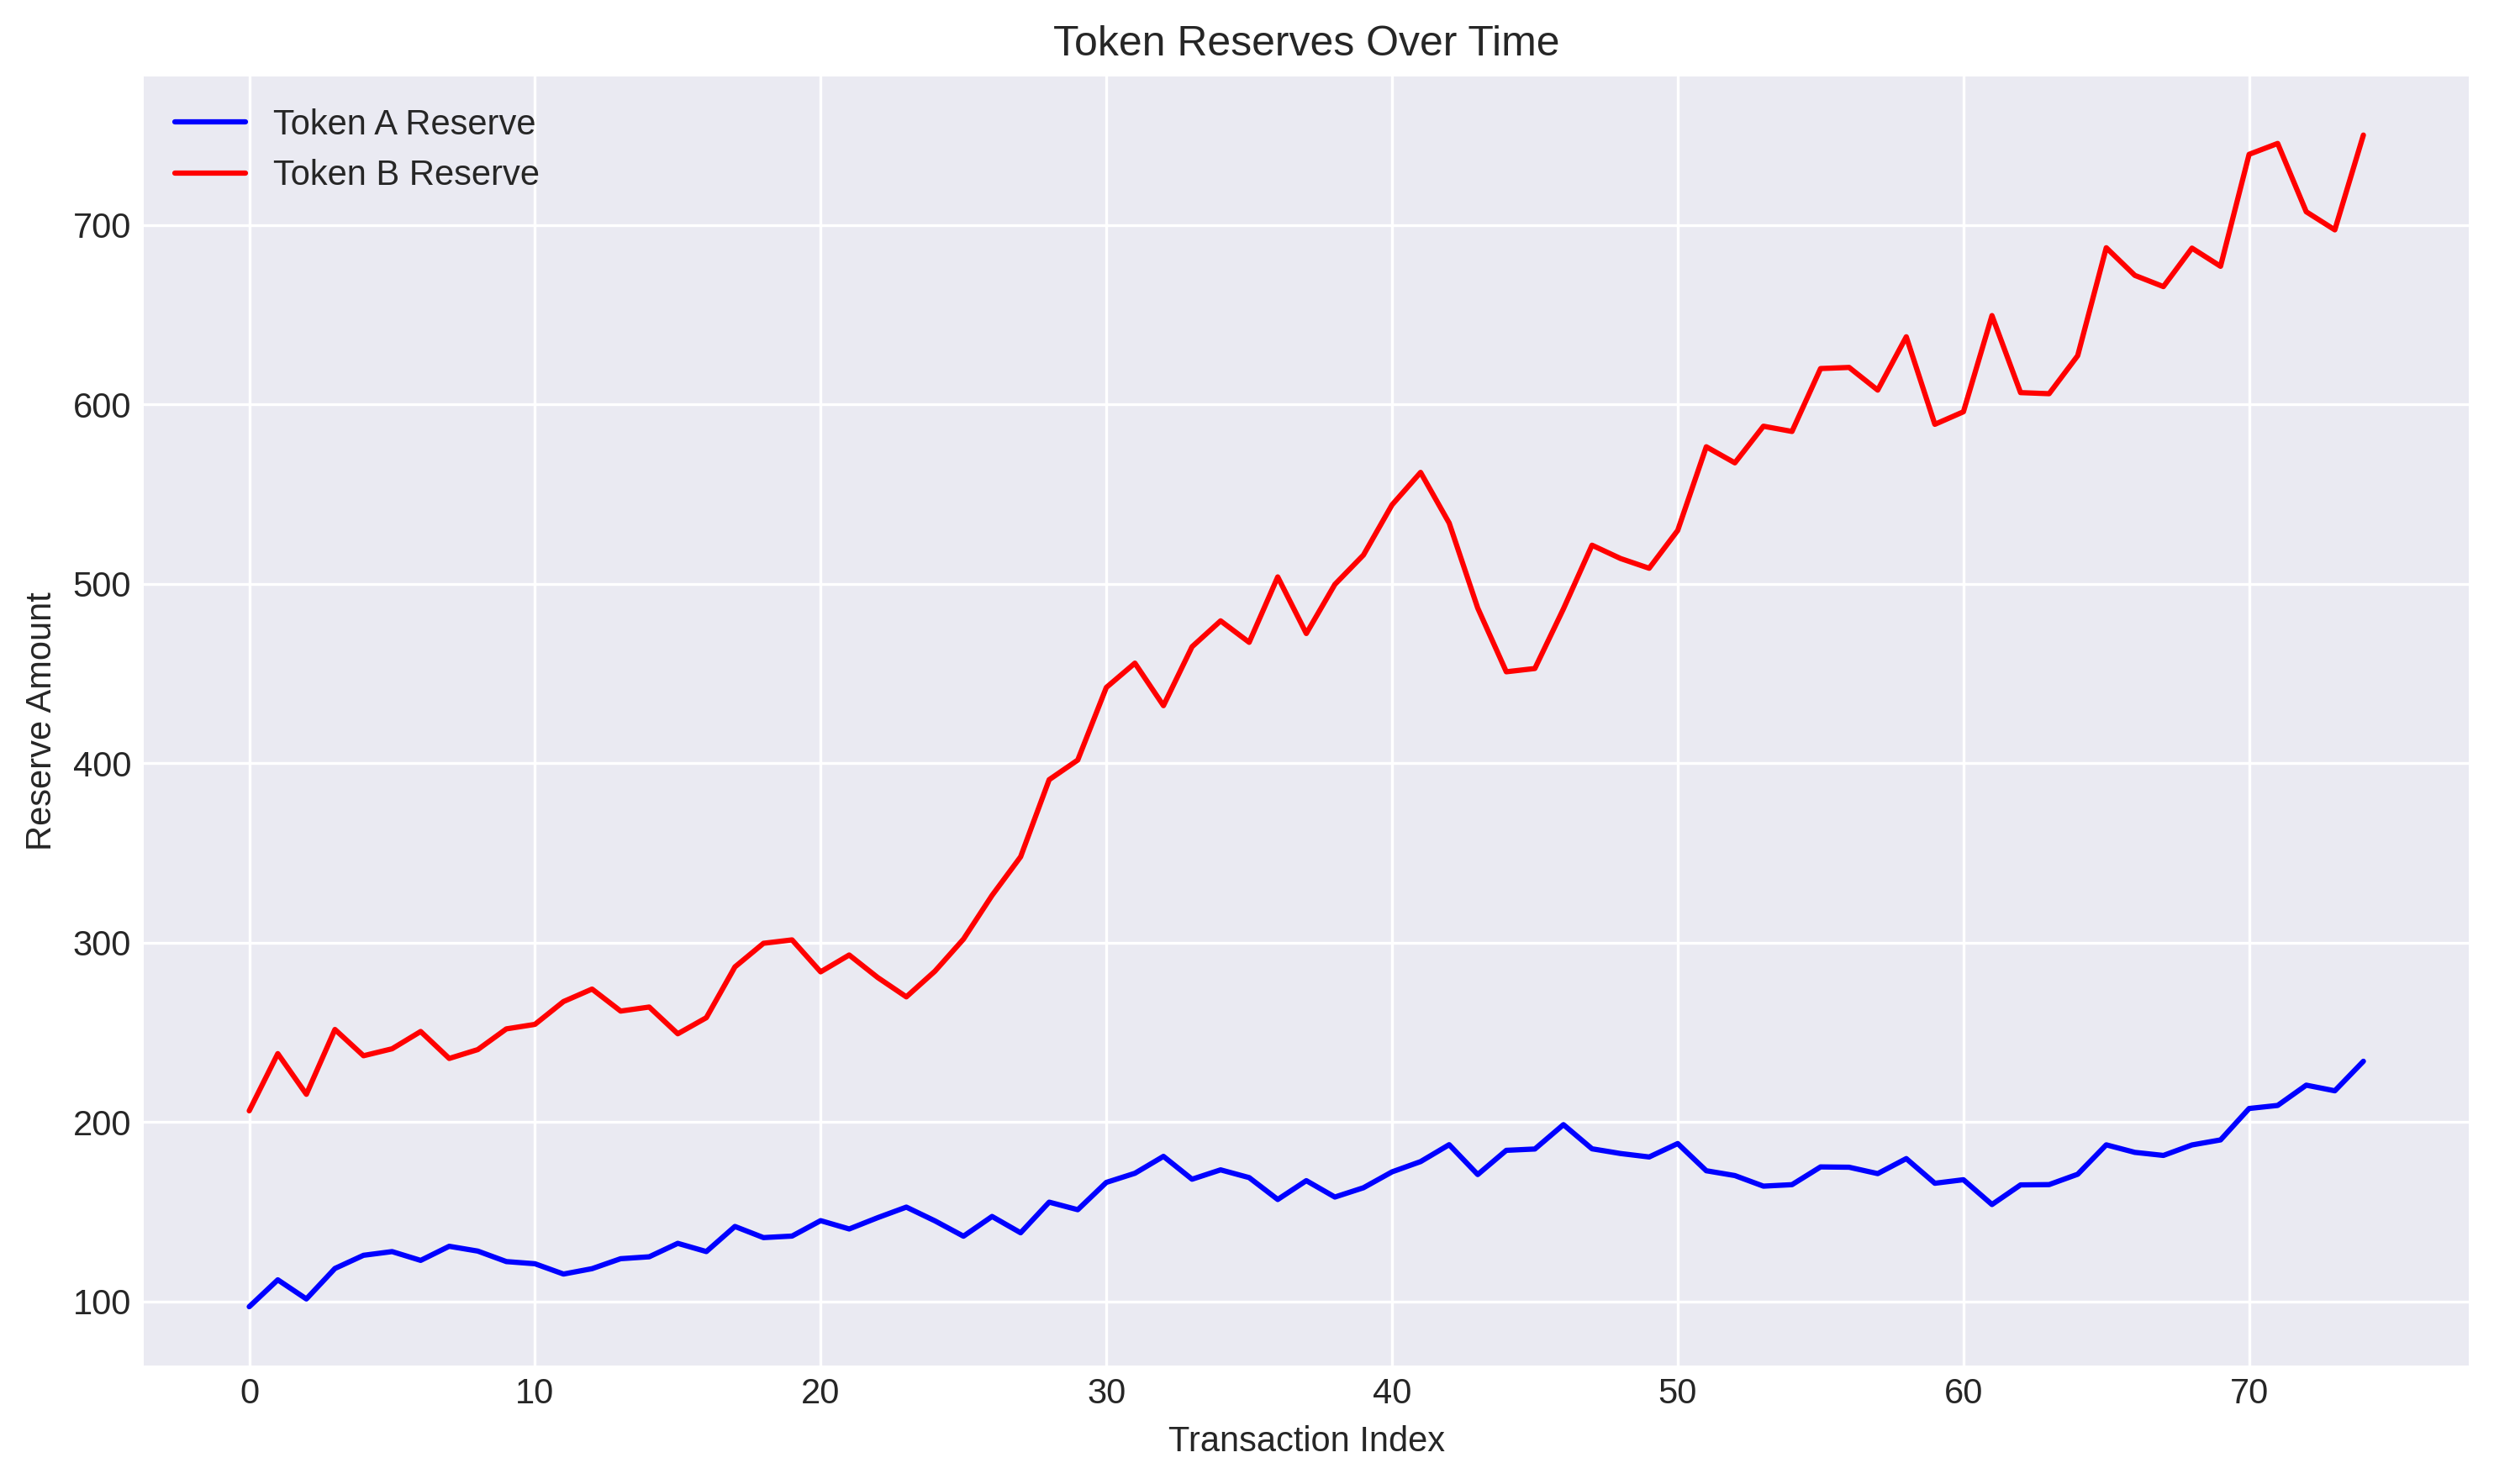
\includegraphics[width=0.9\textwidth]{../task2_plots/reserves.png}
    \caption{Plot of Token Reserves vs. Transaction Index}
    \label{fig:reserves}
\end{figure}

\begin{figure}[H]
    \centering
    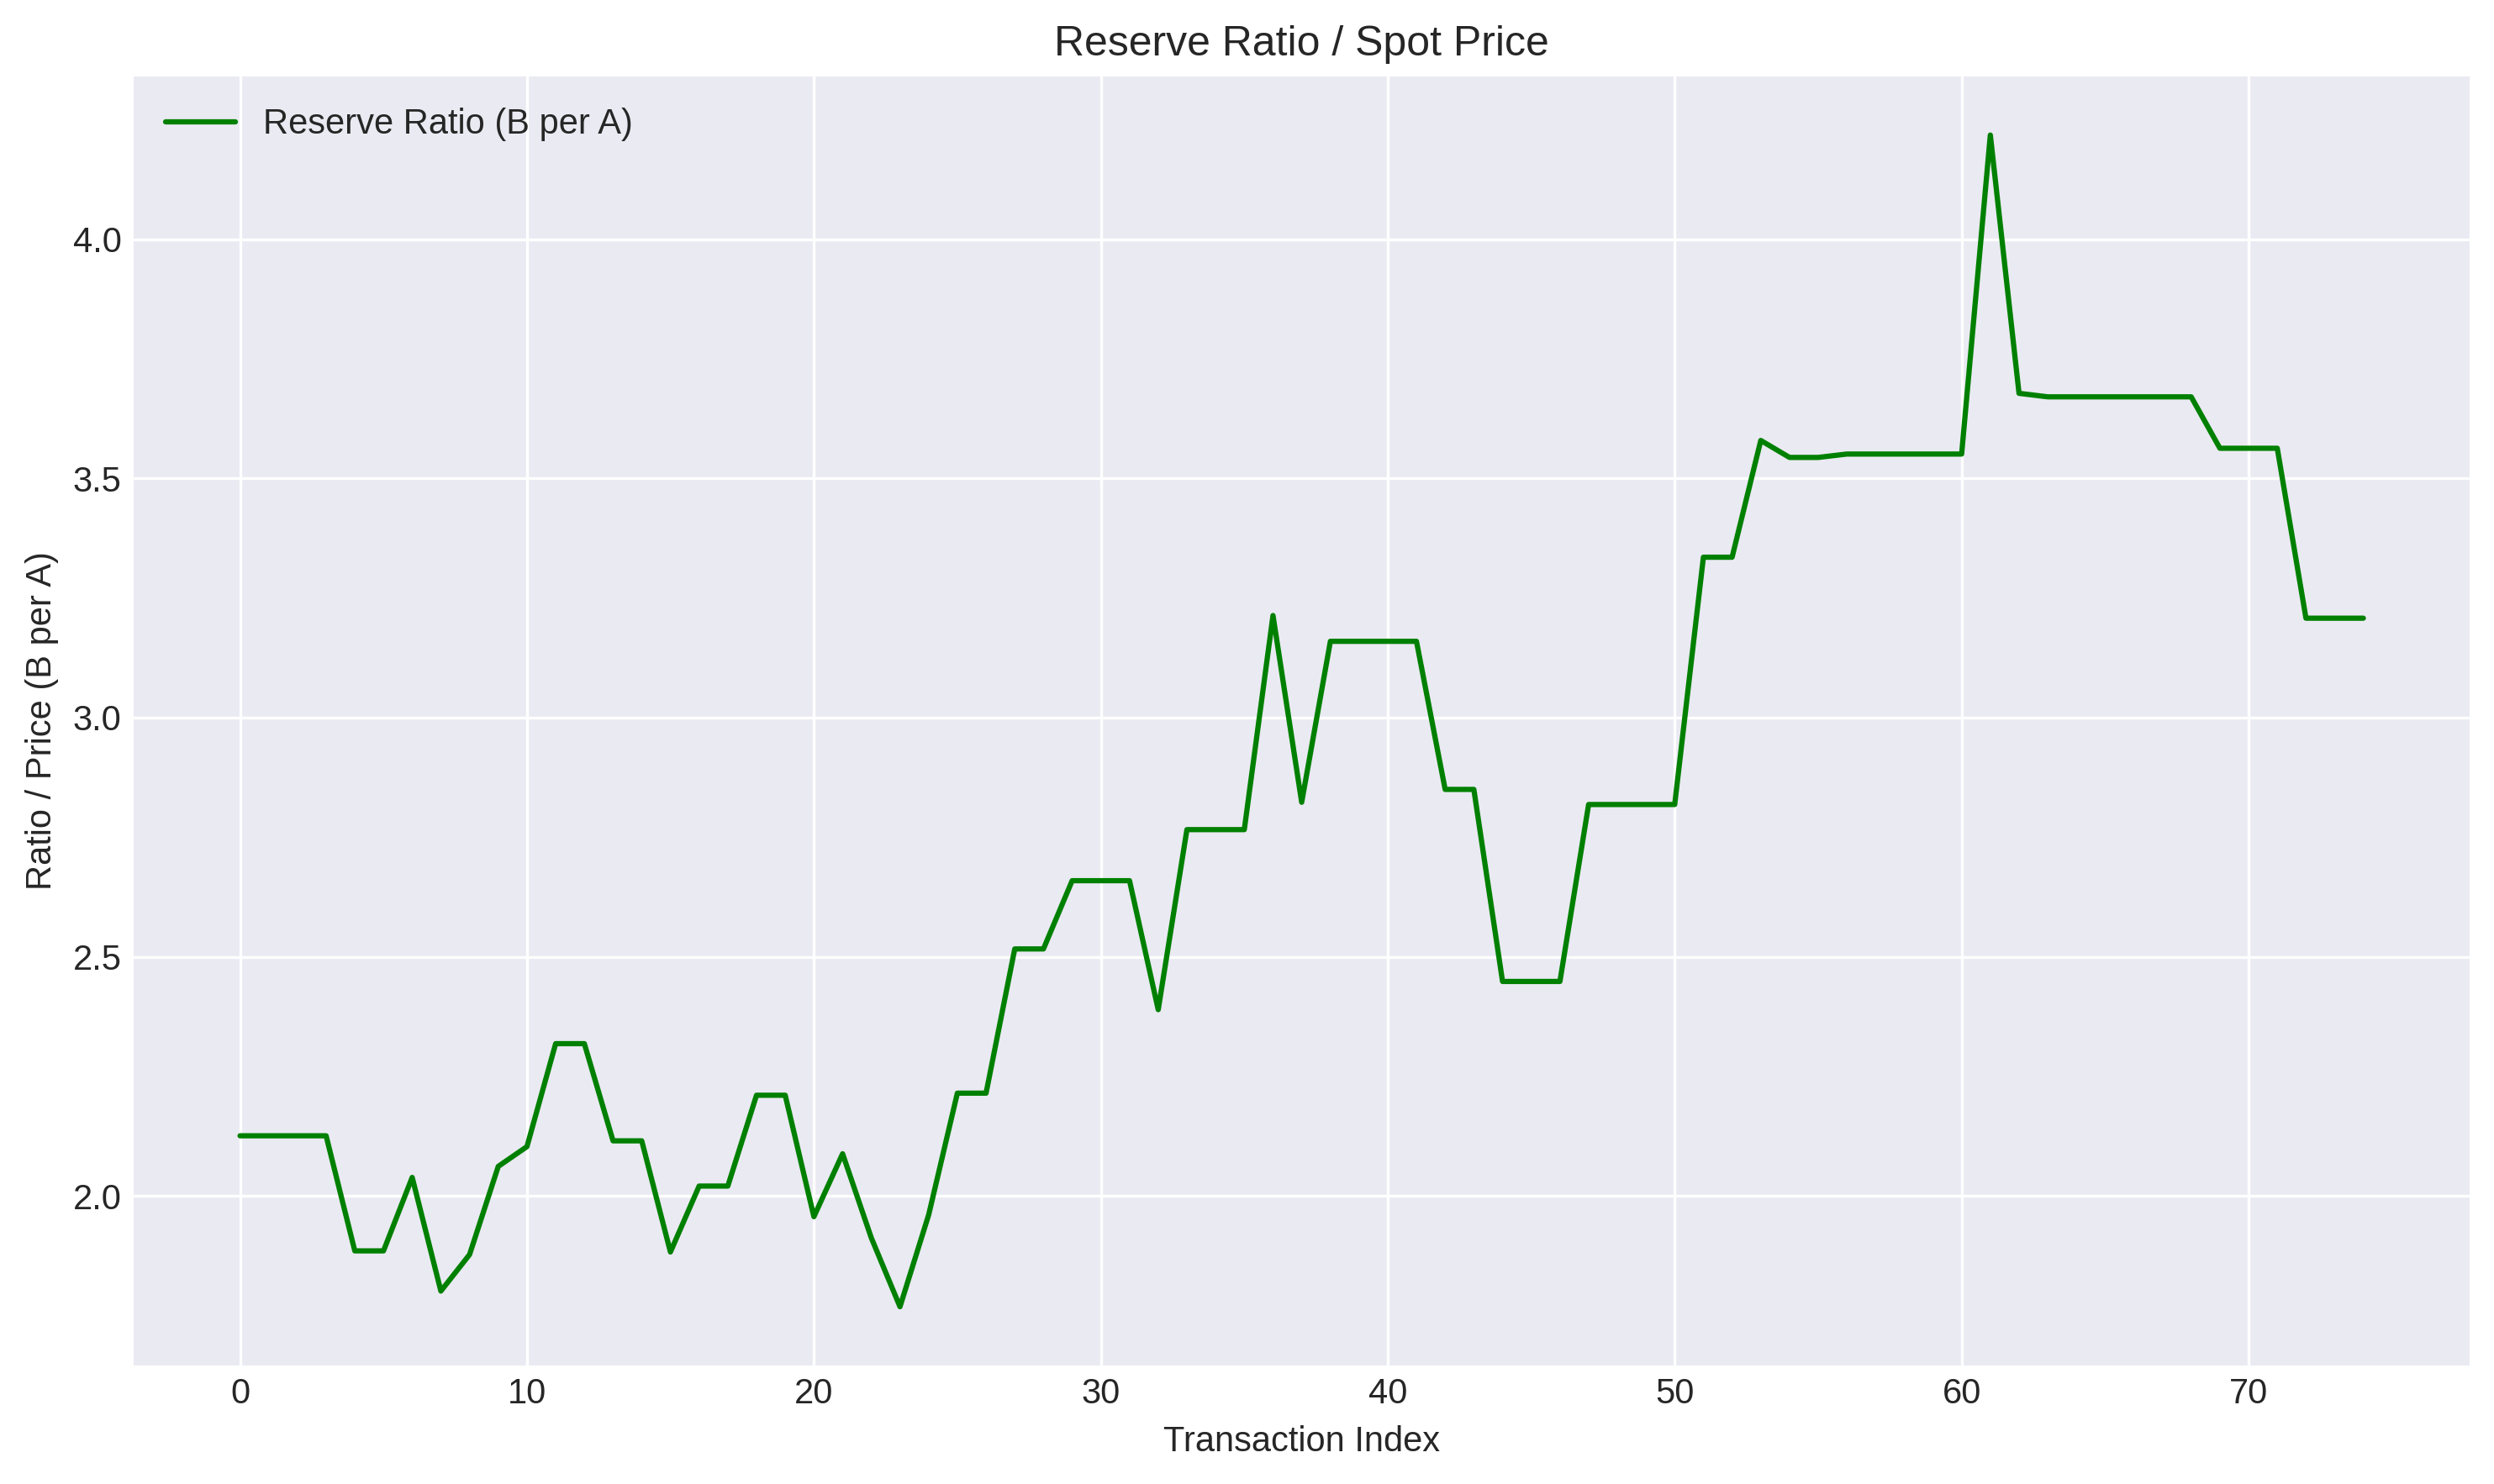
\includegraphics[width=\textwidth]{../task2_plots/reserve_ratio_spot_price.png}
    \caption{Plot of Reserve Ratio / Spot Price vs. Transaction Index}
    \label{fig:ratio}
\end{figure}

\begin{figure}[H]
    \centering
    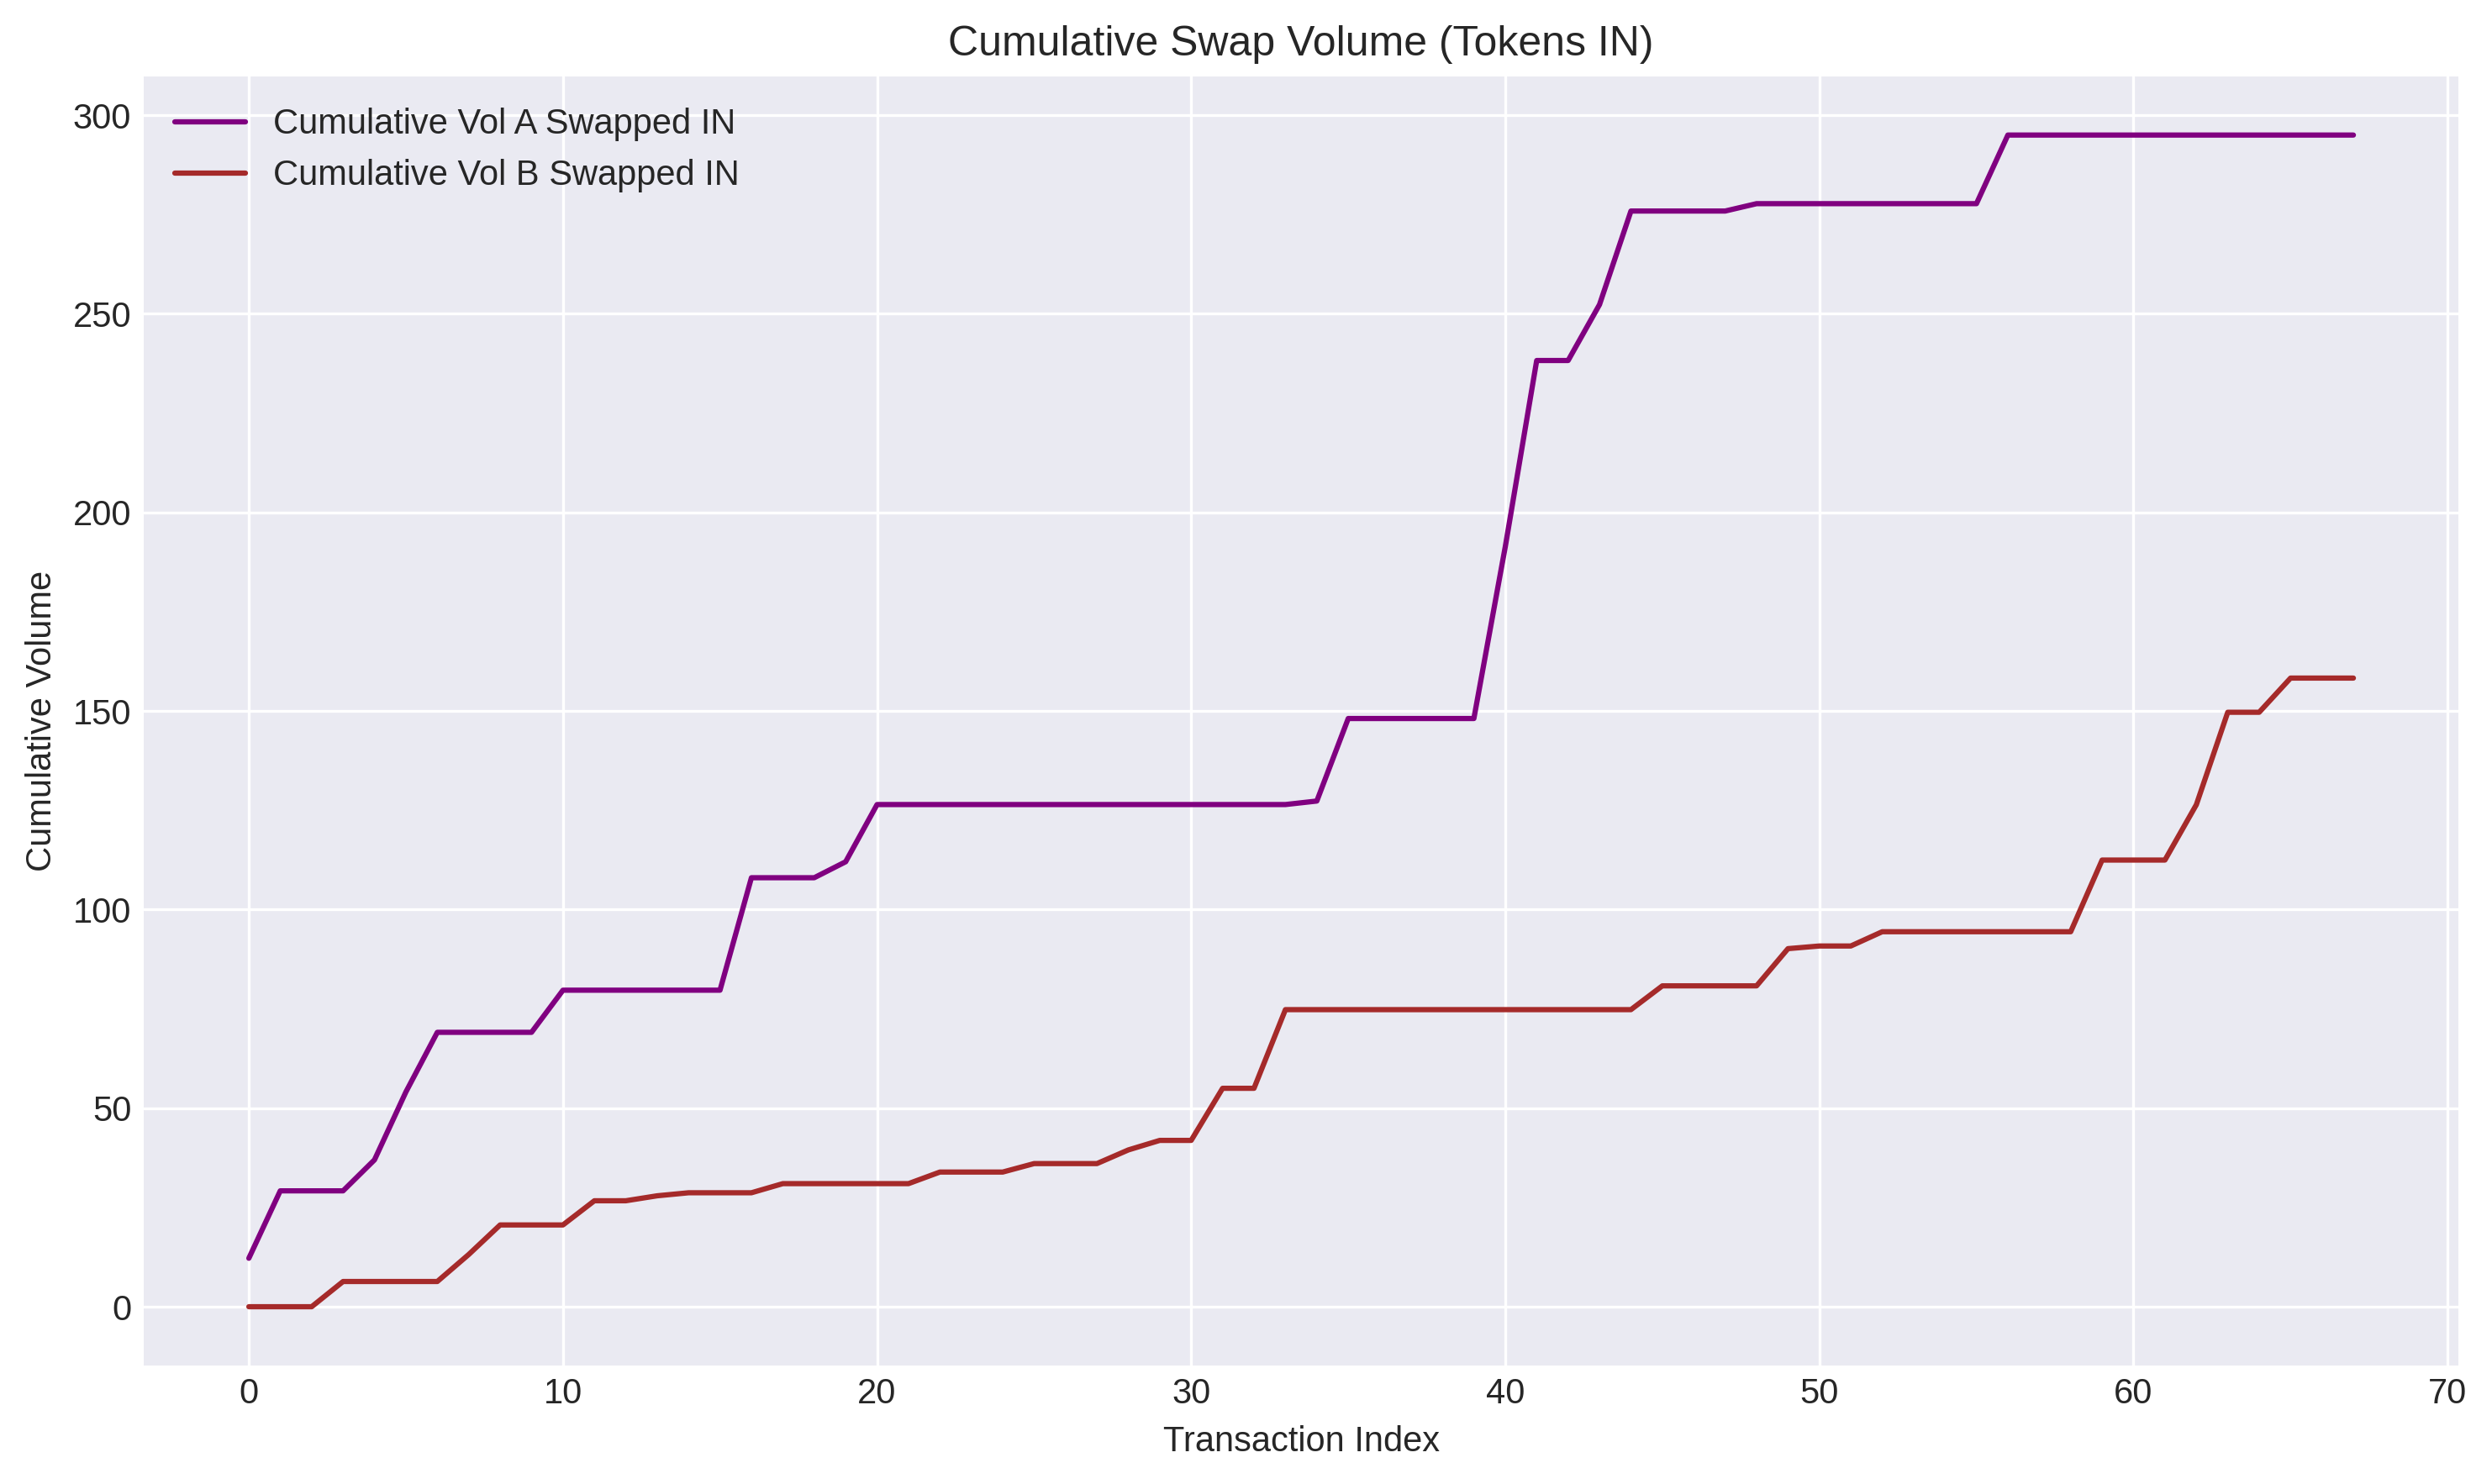
\includegraphics[width=\textwidth]{../task2_plots/swap_volume.png}
    \caption{Plot of Cumulative Swap Volume vs. Transaction Index}
    \label{fig:volume}
\end{figure}

\begin{figure}[H]
    \centering
    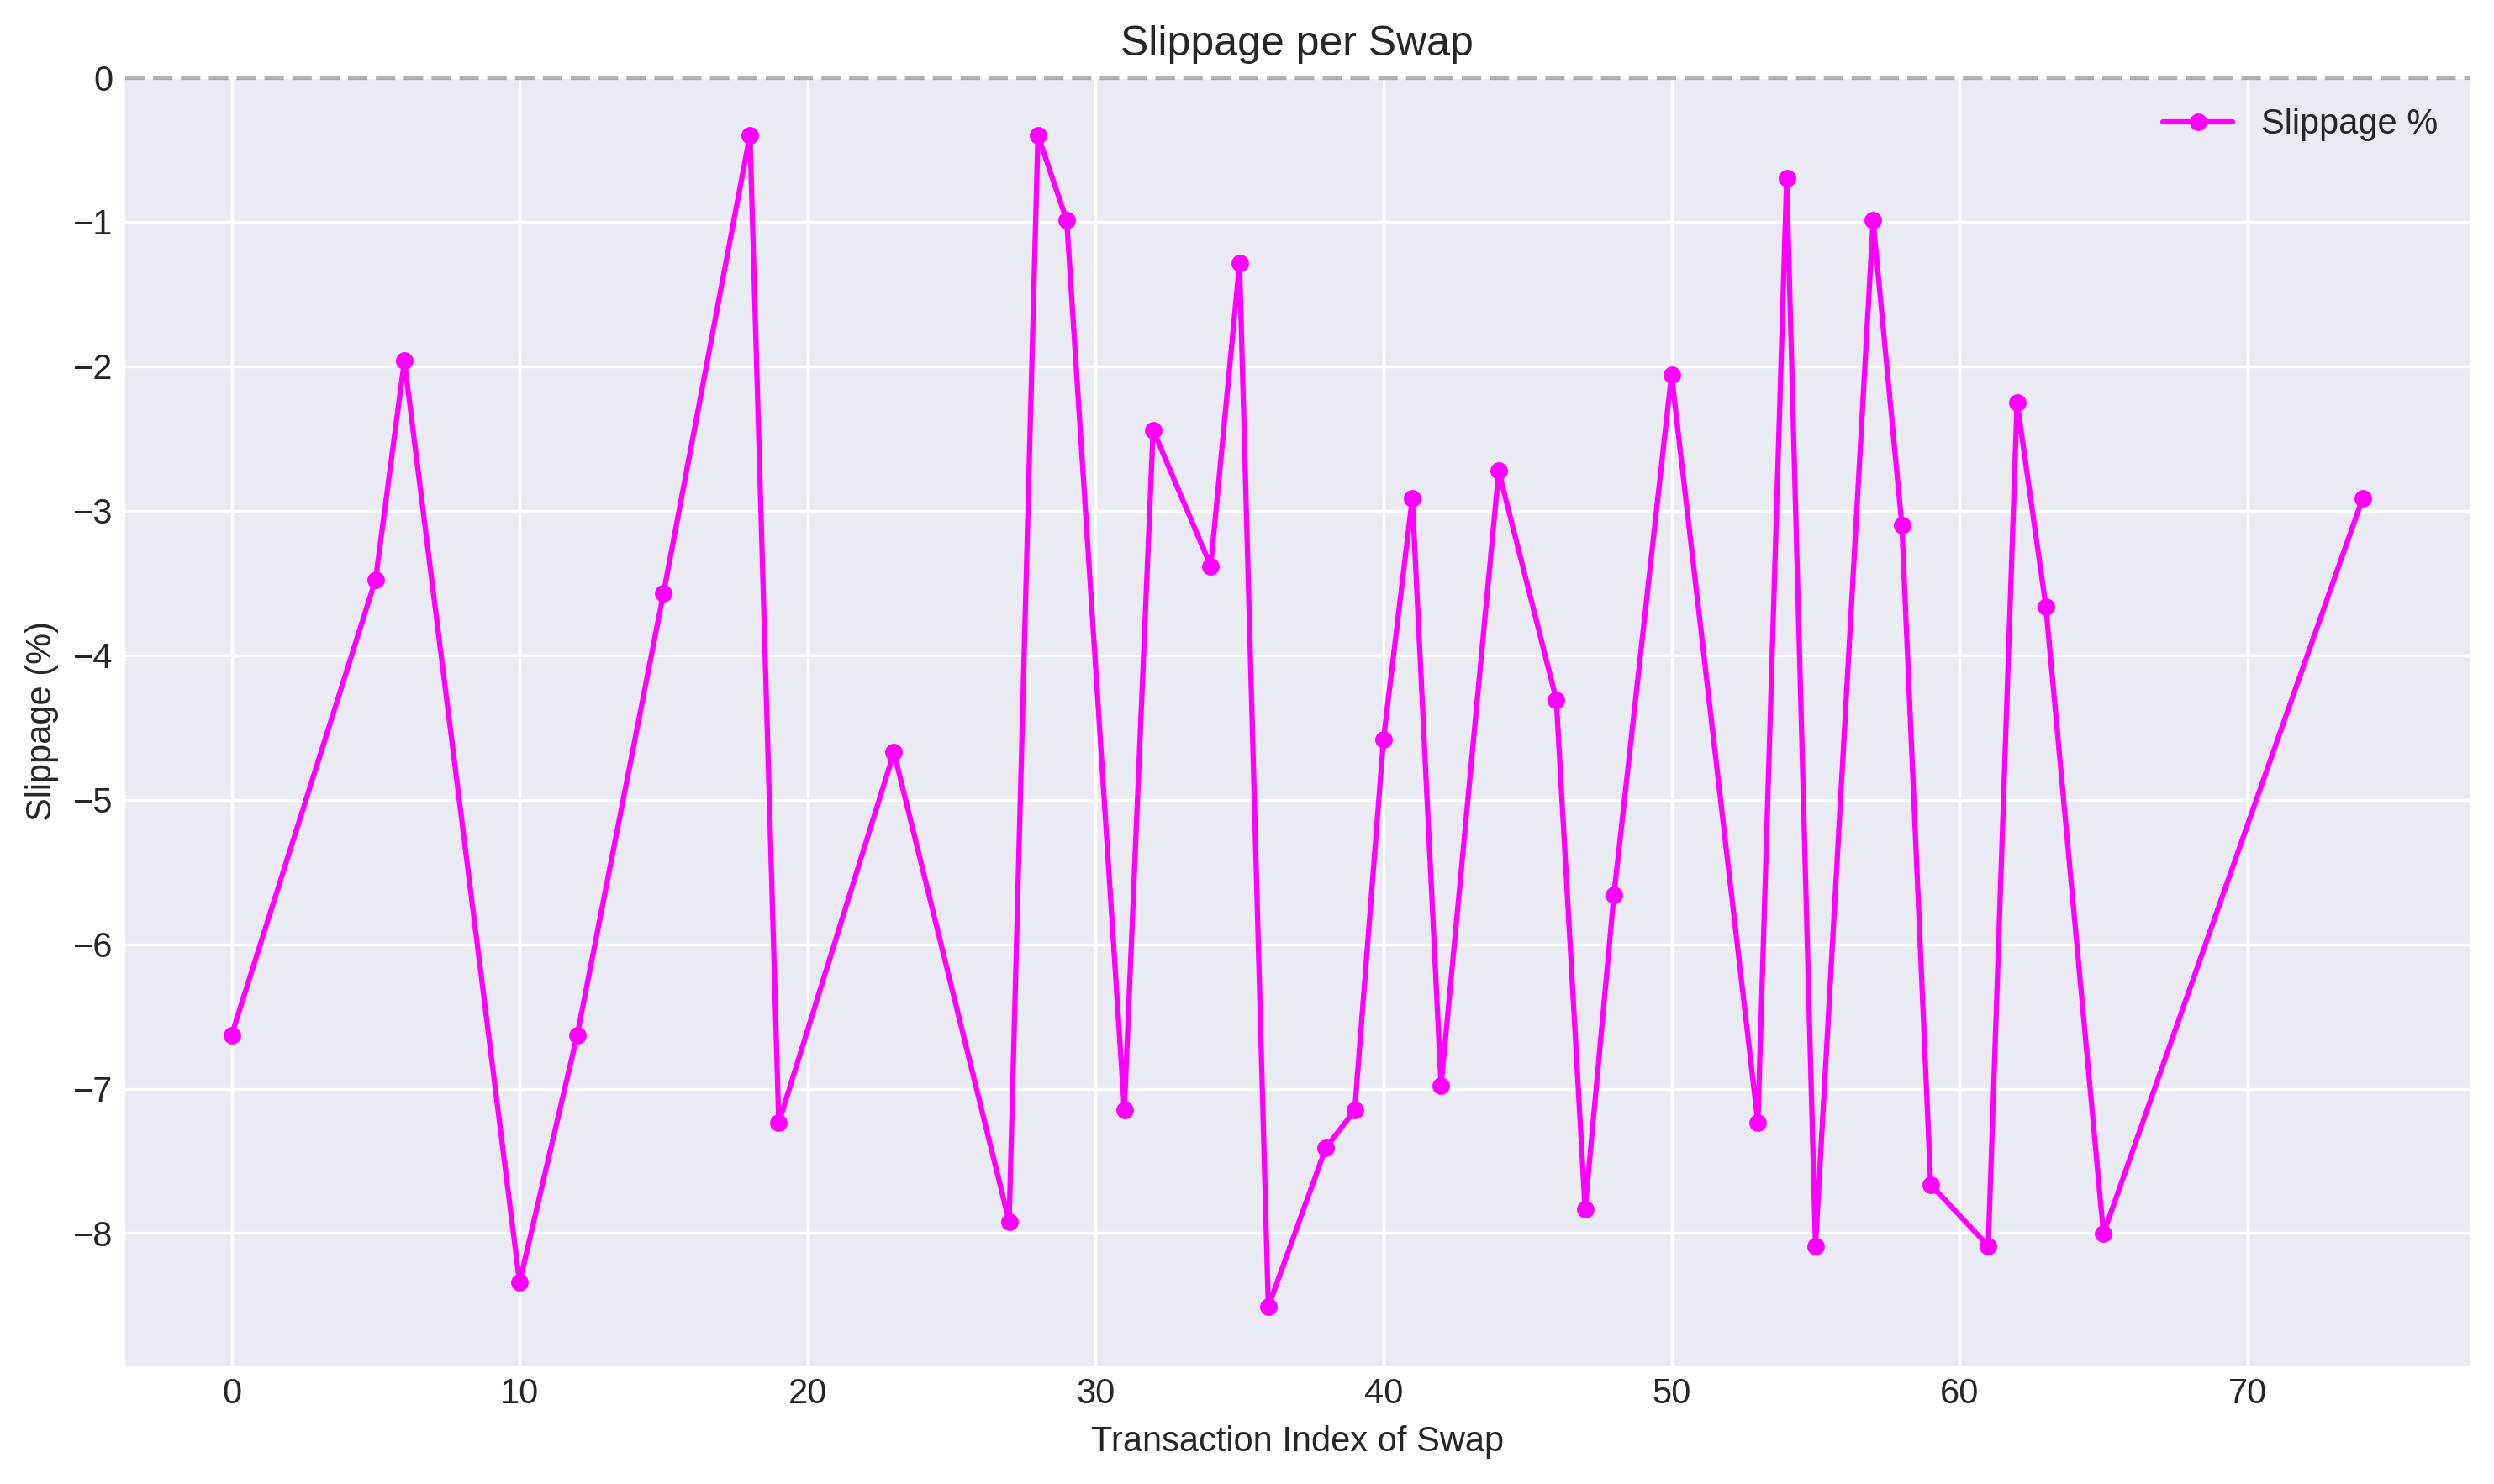
\includegraphics[width=\textwidth]{../task2_plots/slippage.png}
    \caption{Plot of Slippage per Swap vs. Transaction Index}
    \label{fig:slippage}
\end{figure}

\begin{figure}[H]
    \centering
    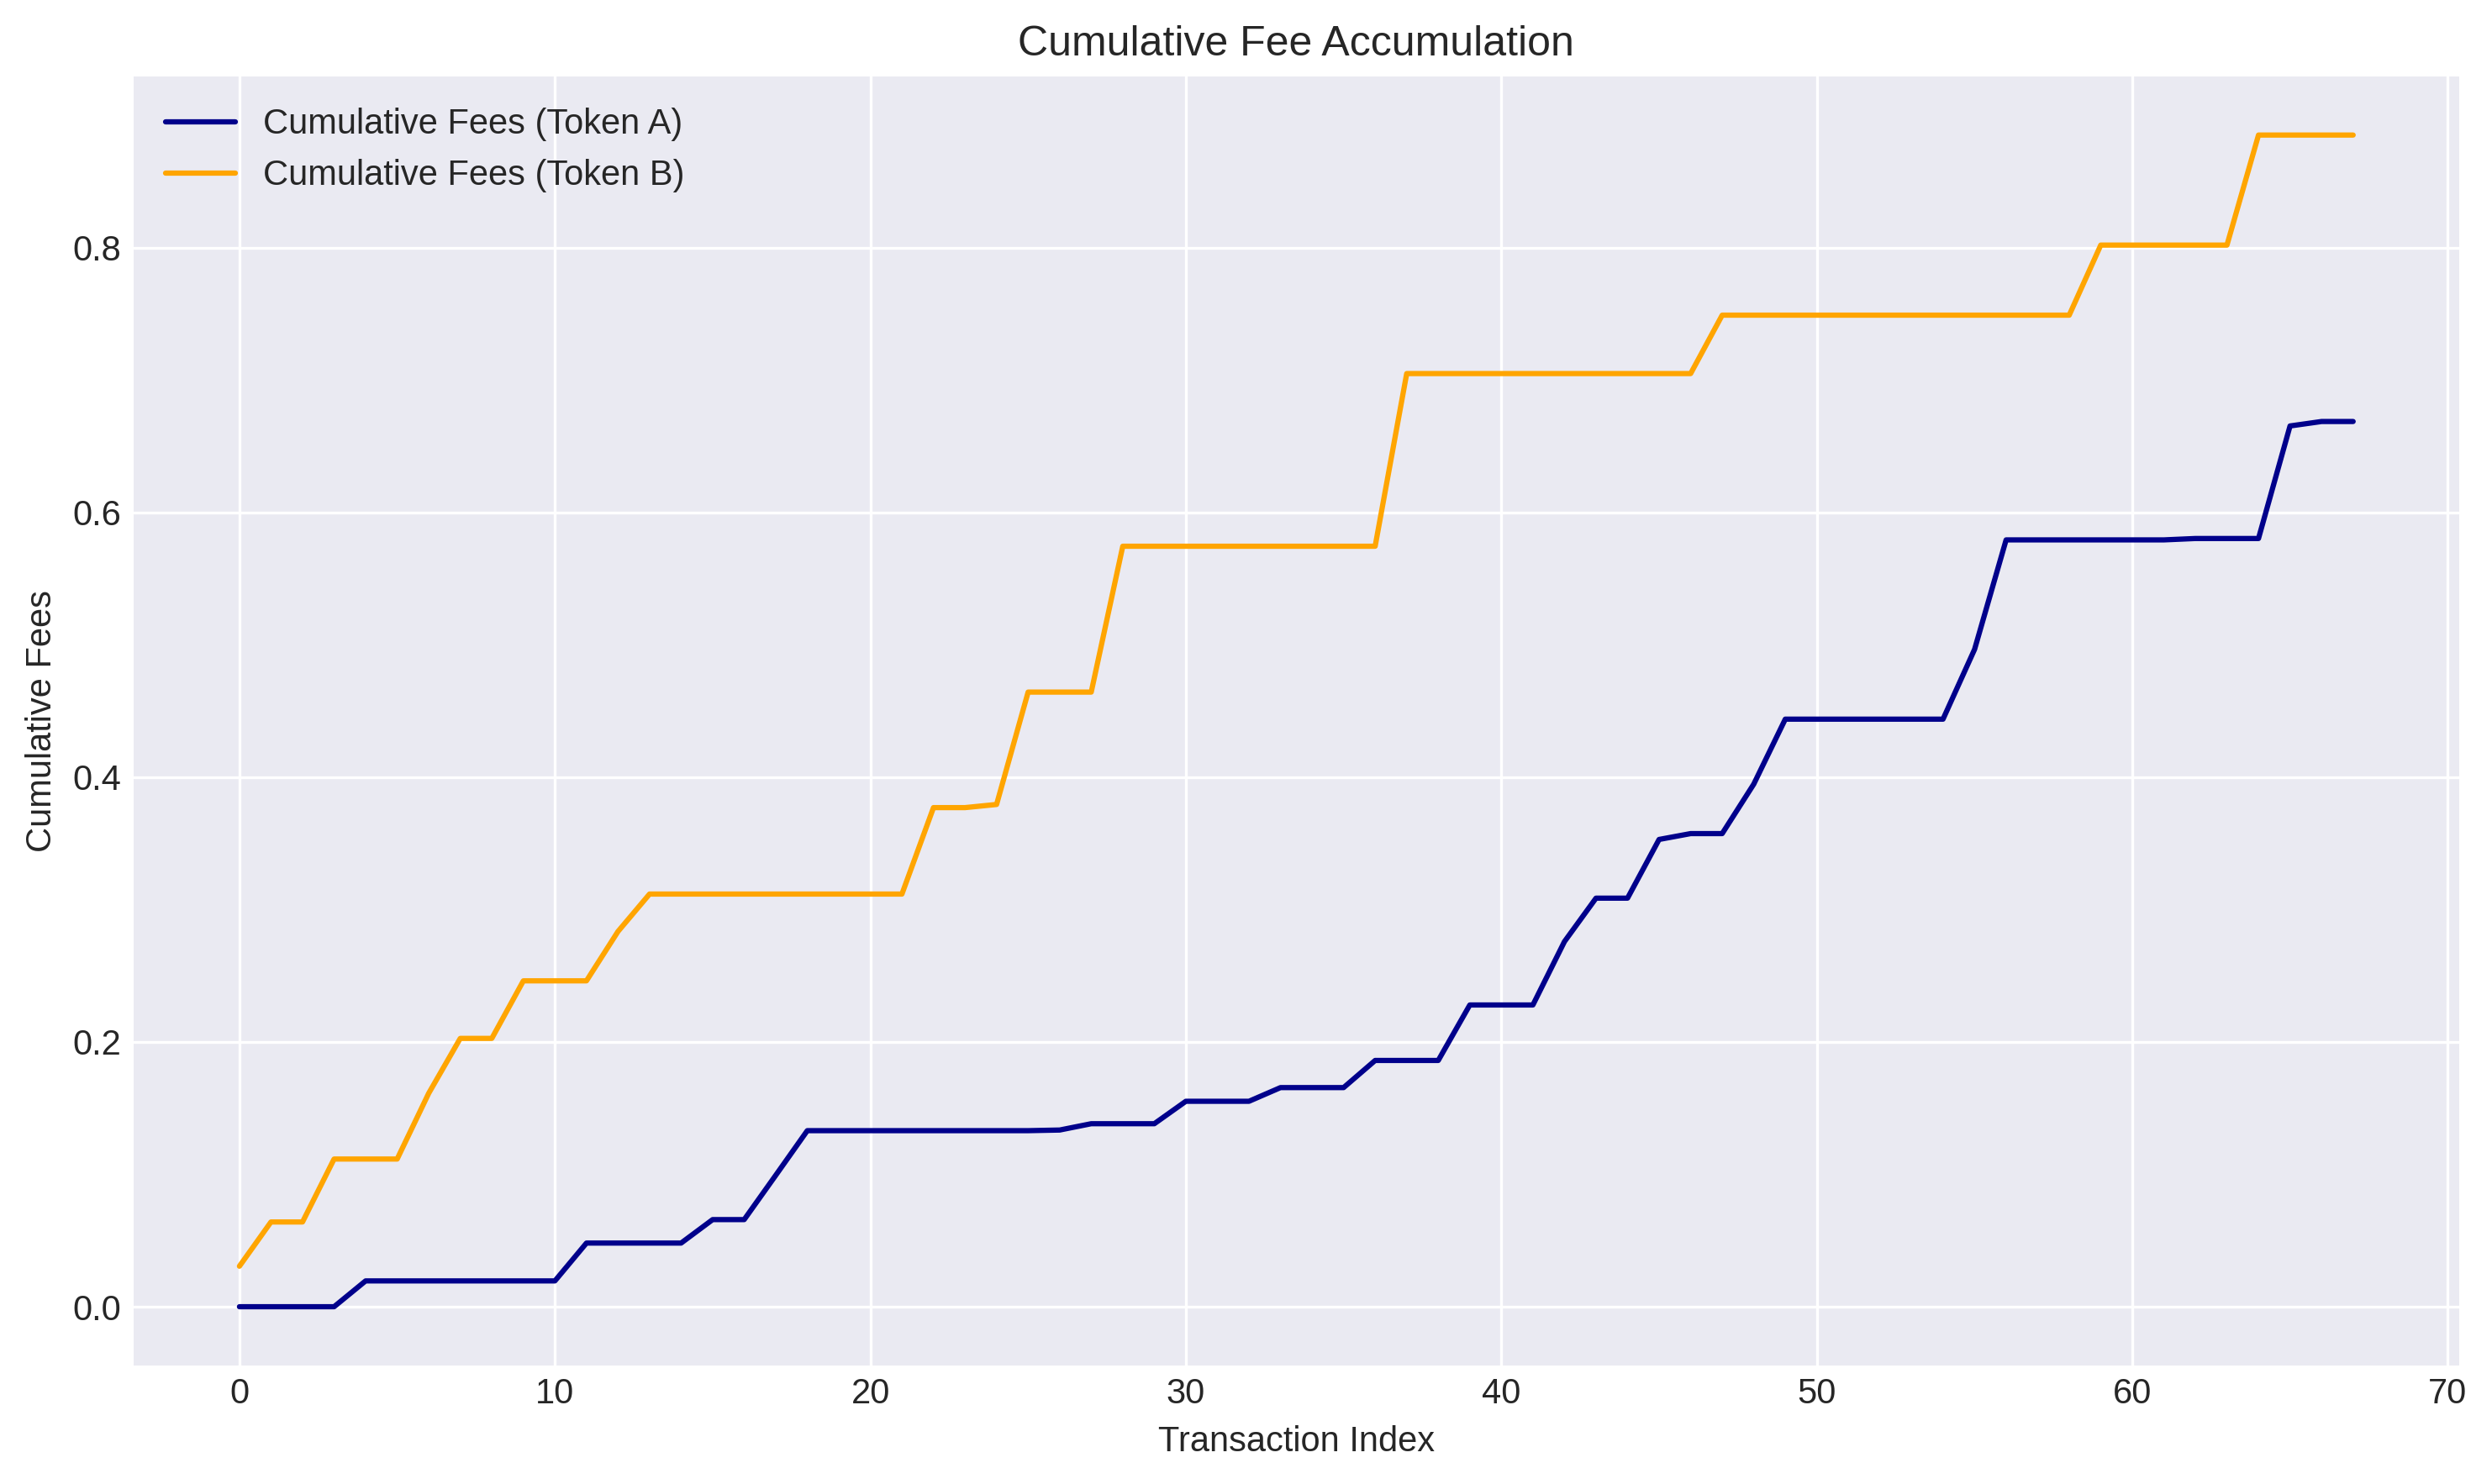
\includegraphics[width=\textwidth]{../task2_plots/fee_accumulation.png}
    \caption{Plot of Cumulative Fee Accumulation vs. Transaction Index}
    \label{fig:fees}
\end{figure}

\begin{figure}[H]
    \centering
    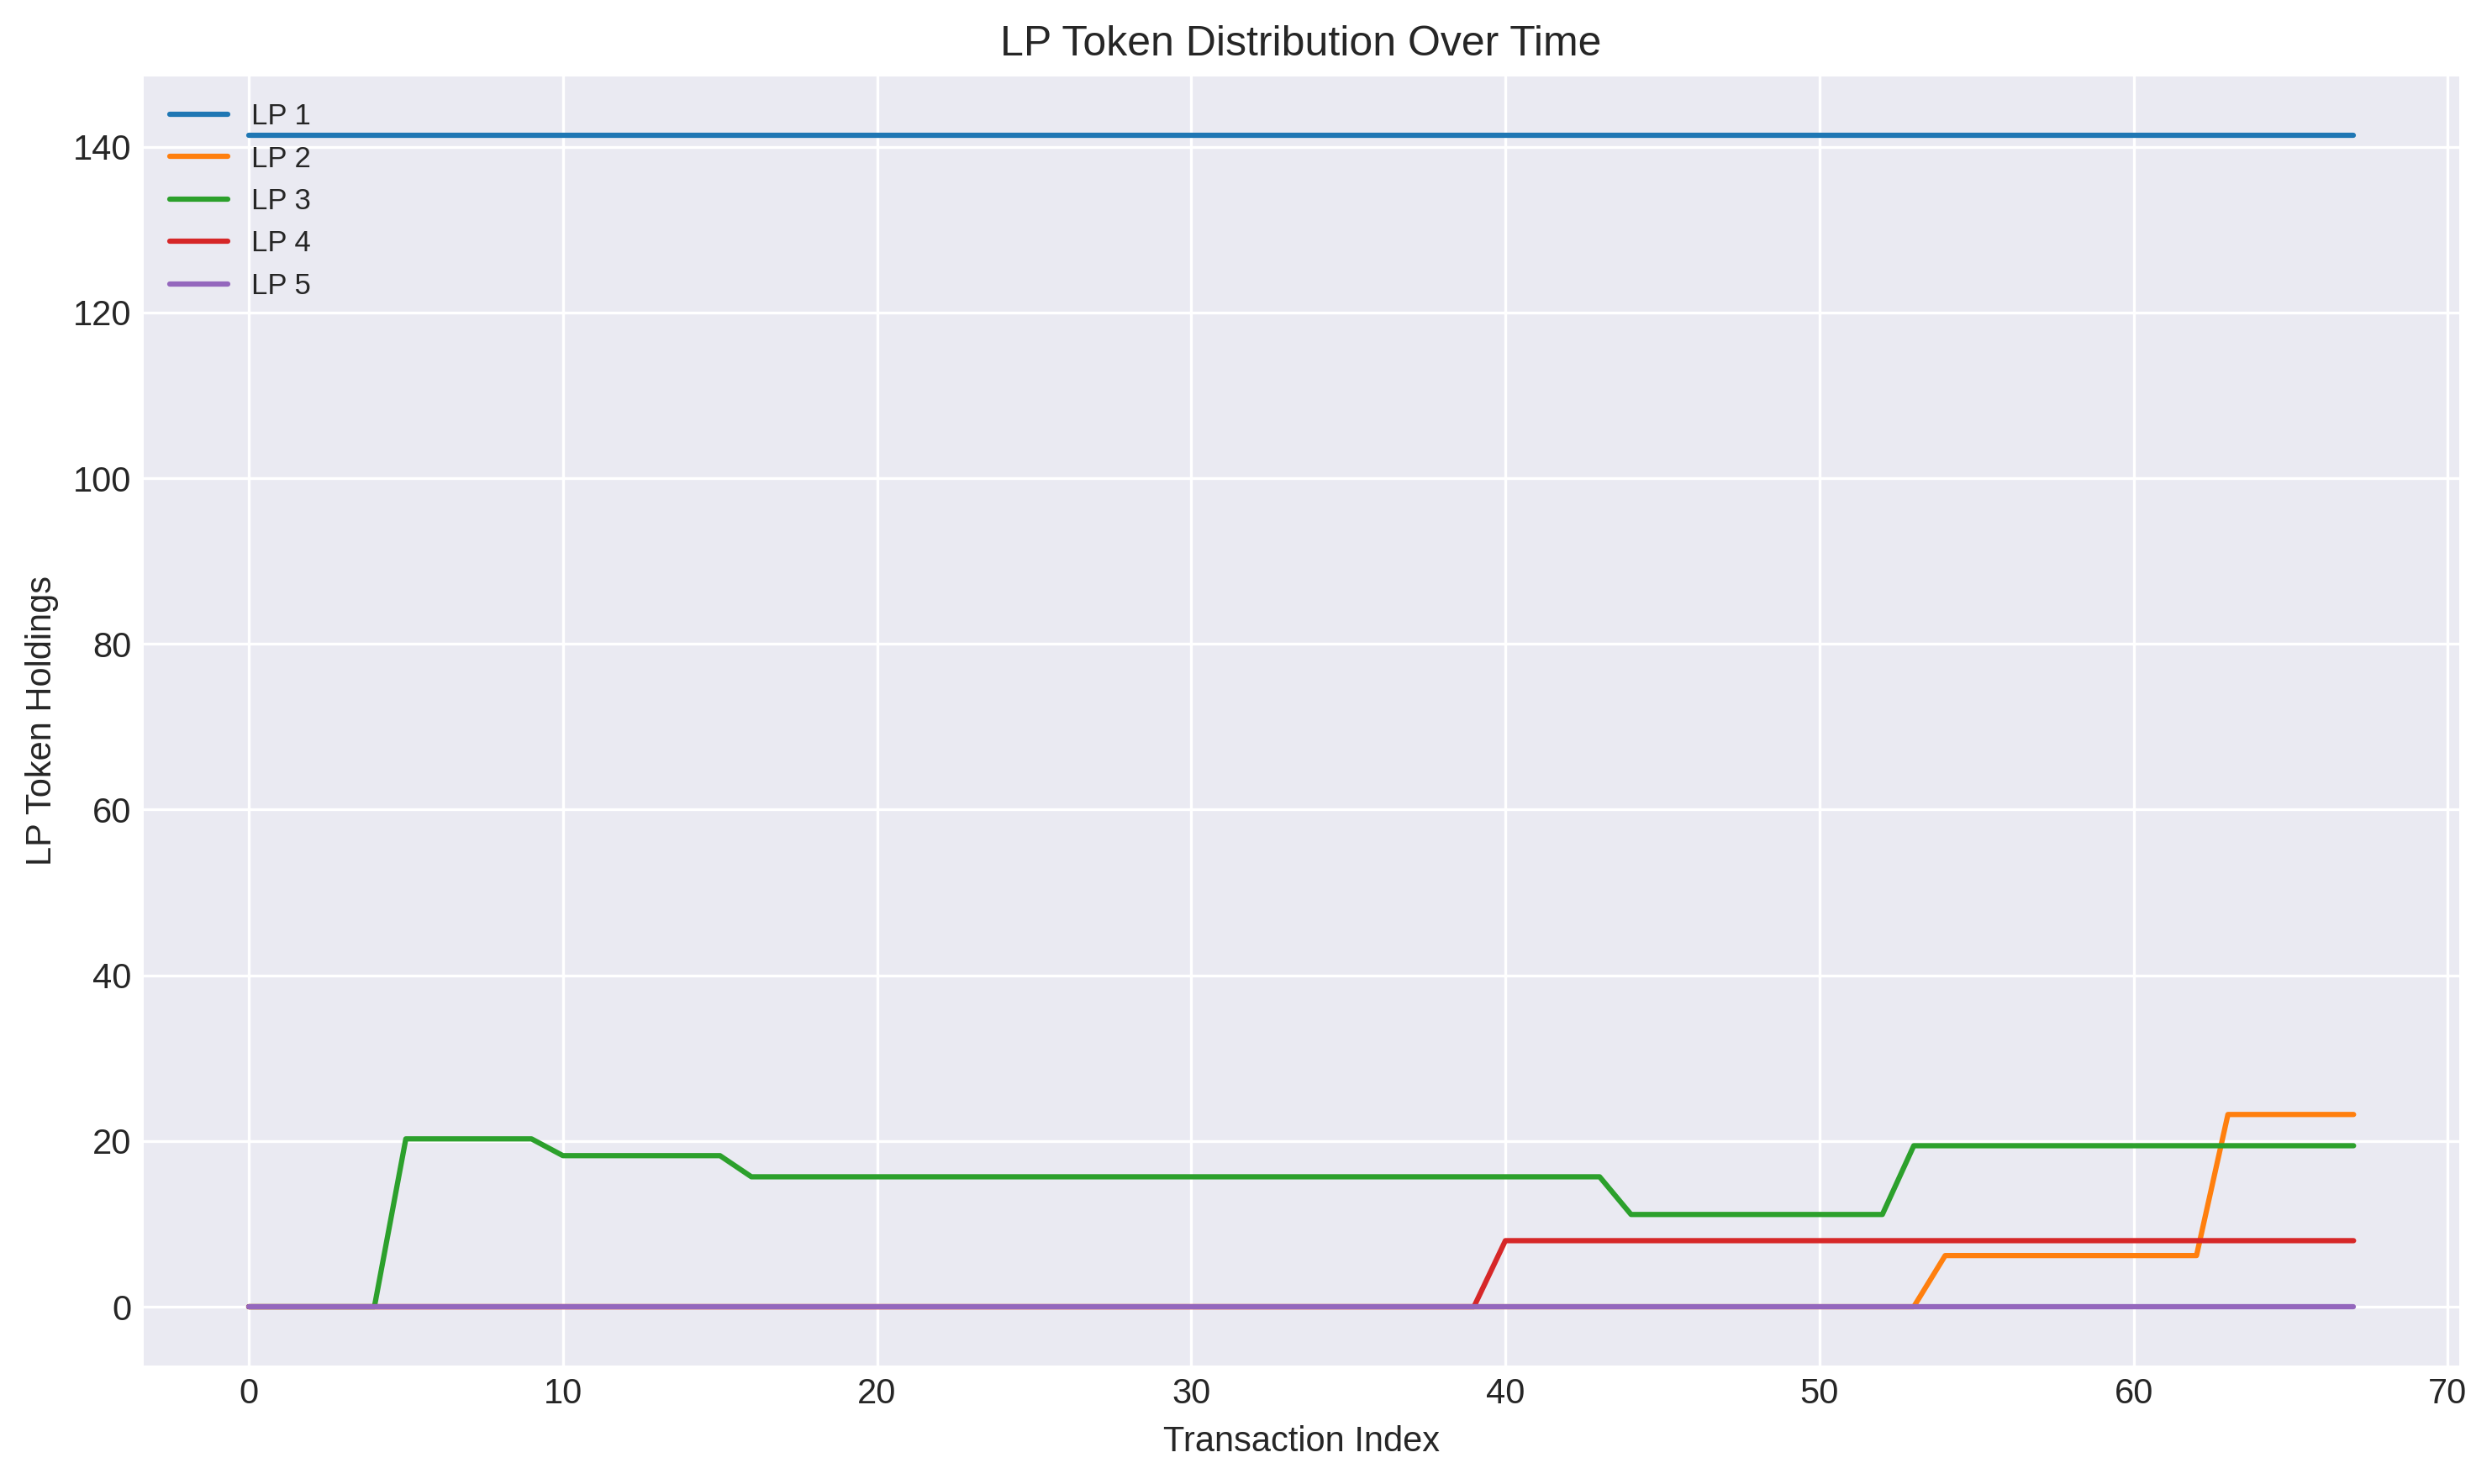
\includegraphics[width=\textwidth]{../task2_plots/lp_distribution.png}
    \caption{Plot of LP Token Distribution vs. Transaction Index (Stacked Area)}
    \label{fig:lp_dist}
\end{figure}


\section{Task 3: Arbitrage Bot Implementation and Simulation}

\subsection{Arbitrage Bot Contract (\texttt{arbitrage.sol})}
An arbitrage bot contract was implemented to exploit price differences between two instances of the previously built DEX.
\begin{itemize}
    \item \textbf{Setup:} The contract stores the addresses of Token A, Token B, DEX1, and DEX2, which are set during deployment. It requires initial funding with both Token A and B to execute trades. It includes `Ownable` for control and withdrawal functions.
    \item \textbf{Price Fetching:} It uses an internal helper function \texttt{getAmountOut} to query the reserves of a specified DEX and predict the output of a potential swap, accounting for the 0.3\% fee and the constant product formula (implicitly estimating price impact).
    \item \textbf{Opportunity Calculation:} The main function \texttt{executeArbitrage} calculates the potential profit for all four arbitrage paths (\(A \rightarrow 1 \rightarrow B \rightarrow 2 \rightarrow A\), \(A \rightarrow 2 \rightarrow B \rightarrow 1 \rightarrow A\), \(B \rightarrow 1 \rightarrow A \rightarrow 2 \rightarrow B\), \(B \rightarrow 2 \rightarrow A \rightarrow 1 \rightarrow B\)) by calling \texttt{getAmountOut} twice for each path.
\end{itemize}

\subsection{Arbitrage Simulation (\texttt{simulate\_arbitrage.js})}
A Javascript script (\texttt{simulate\_arbitrage.js}) was created to test the arbitrage bot.
\begin{itemize}
    \item \textbf{Setup:} The script automates the deployment setup. This includes deploying Token A/B, two separate LP Tokens, two DEX instances (DEX1 and DEX2), transferring ownership of LP Tokens to their respective DEXes, funding an initial LP account (`accounts[1]'), adding initial liquidity to DEX1 and DEX2 with different ratios (e.g., 1A:2B vs 1A:2.1B) to create a price difference, deploying the `Arbitrage` contract linked to the tokens and DEXes, and funding the `Arbitrage' contract with starting capital (e.g., 10 A, 10 B).
    \item \textbf{Scenario 1 (Profitable Arbitrage):} The script calls \texttt{executeArbitrage} on the deployed bot. The console output confirmed that the \texttt{ArbitrageExecuted} event was emitted, and the arbitrage contract's token balance increased, demonstrating a successful profitable execution as required.
    \item \textbf{Scenario 2 (Insufficient Profit):} The script then calls \texttt{setMinProfitThreshold} on the arbitrage contract to set an extremely high threshold. It calls \texttt{executeArbitrage} again. The console output confirmed that no \texttt{ArbitrageExecuted} event was emitted and the contract balances did not change, demonstrating correct non-execution when profit is below the threshold, as required.
\end{itemize}
The simulation successfully demonstrated both required scenarios, which validates the arbitrage bot's functionality.

\section{Task 4: Theory Questions}

\subsection{Q1: LP Token Mint/Burn Permissions}
\textbf{Question:} Which address(es) should be allowed to mint/burn the LP tokens?

\textbf{Answer:} Only the DEX contract address itself should have the permission to mint and burn its corresponding LP tokens. This is crucial for maintaining the integrity of the pool.
Allowing any other address (including the original deployer or individual users) to freely mint or burn LP tokens would break the fundamental link between the LP tokens and the actual reserves held in the pool, enabling theft or manipulation. In our implementation, this is achieved by making the \texttt{LPToken} contract \texttt{Ownable} and transferring ownership to the deployed \texttt{DEX} contract. The \texttt{mint} and \texttt{burn} functions in \texttt{LPToken} have the \texttt{onlyOwner} modifier.

\subsection{Q2: DEXs fair playing ground?}
\textbf{Question:} In what way do DEXs level the playing ground between a powerful and resourceful trader (HFT/institutional investor) and a lower resource trader (retail investors, like you and me!)?

\textbf{Answer:} DEXs offer several features that can partially level the playing ground compared to centralized exchanges (CEXs), although advantages for resourceful traders still exist:
\begin{itemize}
    \item \textbf{Transparency:} All trading rules (the AMM smart contract code) and transaction history are publicly visible on the blockchain. There are no hidden order books or special access privileges (like co-location for HFTs on CEXs). Everyone interacts with the same contract under the same rules.
    \item \textbf{Permissionless Access:} Anyone with a wallet can interact with the DEX; there are typically no complex onboarding processes, API access tiers, or preferential treatment based on trading volume that large players might exploit on CEXs.
    \item \textbf{Deterministic Execution (Mostly):} AMM logic is deterministic based on pool reserves. While miners can influence transaction order, the outcome of a specific swap against a specific pool state (before the swap) is predictable by the formula.
    \item \textbf{Reduced Counterparty Risk:} Users typically retain custody of their assets until the point of trade (interacting via their own wallet), reducing the risk associated with exchange hacks or insolvency prevalent in CEXs.
\end{itemize}
However, resourceful traders still have advantages in DeFi through concepts like Miner Extractable Value (MEV), superior infrastructure for monitoring mempools and executing faster, and the capital to perform large trades or provide significant liquidity.

\subsection{Q3: Miner Advantage (MEV)}
\textbf{Question:} Suppose there are many transaction requests to the DEX sitting in a miner's mempool. How can the miner take undue advantage of this information? Is it possible to make the DEX robust against it?

\textbf{Answer:} Miners (or validators in Proof-of-Stake) have visibility into the pool of pending transactions (mempool) before they are included in a block. They also typically have the power to arbitrarily order (and sometimes insert/censor) transactions within the block they produce. This creates opportunities for Miner Extractable Value (MEV) that exploit DEX users:
\begin{itemize}
    \item \textbf{Front-running:} A miner sees a large user swap incoming (e.g., buying Token B with Token A) that will increase the price of Token B. The miner inserts their own transaction just before the user's swap to buy Token B at the lower price. After the user's large swap pushes the price up, the miner inserts another transaction to sell their Token B at the new, higher price, capturing a risk-free profit.
    \item \textbf{Back-running:} A miner sees a transaction that creates an arbitrage opportunity (e.g., adding liquidity that significantly changes the price relative to another DEX). They execute the user's transaction and immediately insert their own transaction after it to capture the arbitrage profit before anyone else can.
    \item \textbf{Sandwich Attack:} A combination where the miner places a buy order just before the user's buy order (front-running) and a sell order just after it, profiting from the price impact caused by the user's trade.
\end{itemize}
Making a DEX completely robust against MEV is extremely difficult, as miners fundamentally control block production. However, strategies exist to mitigate it:
\begin{itemize}
    \item \textbf{Slippage Tolerance:} Users setting tight slippage tolerances on their swaps can limit the potential profit from sandwich attacks, causing the second leg of the attack to fail.
    \item \textbf{Batch Auctions/Order Matching:} Some DEX designs move away from instant AMM execution and use batch auctions (collecting orders over a short period and settling them at a uniform clearing price) which makes front-running harder.
    \item \textbf{MEV-aware Protocols/Relays:} Services like Flashbots allow users to submit transactions privately to miners, bypassing the public mempool. Miners participating in these systems can execute bundles atomically, potentially preventing front-running by others but still allowing the miner to capture MEV internally or through auctions.
    \item \textbf{Encrypted Mempools:} Future solutions involve encrypting transactions in the mempool so miners cannot see the content until after the block order is committed.
\end{itemize}
The simple AMM in this assignment is vulnerable to these MEV strategies.

\subsection{Q4: Gas Fees Influence}
\textbf{Question:} We have left out a very important dimension on the feasibility of this smart contract the gas fees! Every function call needs gas. How does gas fees influence economic viability of the entire DEX and arbitrage?

\textbf{Answer:} Gas fees are a critical factor in the economic viability of DEXs and arbitrage:
\begin{itemize}
    \item \textbf{DEX Viability (User Perspective):} High gas fees can make swapping small amounts uneconomical. If the gas cost for a swap transaction (which can be significant due to complex AMM calculations and storage updates) is a large percentage of the trade value, users are deterred. This particularly affects smaller retail traders. DEXs on Layer 1 blockchains with high gas fees (like Ethereum mainnet during congestion) become less attractive compared to CEXs or DEXs on cheaper Layer 2 solutions.
    \item \textbf{DEX Viability (LP Perspective):} Adding or removing liquidity also costs gas. LPs need to earn enough in trading fees (the 0.3\% in this case) over time to cover the gas costs of their deposit and withdrawal transactions, plus compensate for impermanent loss risk, to be profitable. High gas fees reduce LP profitability, potentially leading to lower liquidity.
    \item \textbf{Arbitrage Viability:} Arbitrage opportunities often involve small price discrepancies. An arbitrage bot must calculate if the potential profit from exploiting a price difference across two DEXs is greater than the combined gas cost of executing the necessary transactions (at least two swaps, plus approvals if needed). During high gas periods, many small arbitrage opportunities become unprofitable, allowing price discrepancies between venues to persist for longer. Arbitrage bots often compete by using sophisticated gas price strategies to ensure execution while minimizing cost.
\end{itemize}

\subsection{Q5: Gas Fee Advantages}
\textbf{Question:} Could gas fees lead to undue advantages to some transactors over others? How?

\textbf{Answer:} Yes, gas fees can definitely create advantages, primarily favoring those with more capital or sophisticated infrastructure:
\begin{itemize}
    \item \textbf{Priority Gas Auctions (PGAs):} When network congestion is high, users compete for block space by bidding higher gas prices. Wealthy traders or bots (like front-runners or arbitrageurs) can afford to pay significantly higher gas prices to ensure their transactions are processed faster and included before others. This allows them to consistently capture time-sensitive opportunities (like arbitrage or front-running) before retail users whose transactions might be stuck pending due to lower gas prices.
    \item \textbf{Transaction Ordering:} Miners/validators are incentivized to include transactions with higher gas prices first. This gives an advantage to those who can pay more for priority, effectively allowing them to ```cut in line" in the mempool.
    \item \textbf{Economic Exclusion:} As mentioned in Q4, high base gas fees can simply make certain actions (small swaps, frequent LP adjustments) economically infeasible for users with limited capital, while remaining viable for larger players. This restricts participation for smaller users.
    \item \textbf{MEV Exploitation:} Actors specifically searching for MEV opportunities are often willing to pay very high gas fees (sometimes even exceeding the direct arbitrage profit, if they can chain MEV opportunities) to guarantee execution and front-run others.
\end{itemize}

\subsection{Q6: Minimizing Slippage}
\textbf{Question:} What are the various ways to minimize slippage (as defined in 4.2) in a swap? [cite: 69]

\textbf{Answer:} Slippage in an AMM swap is the difference between the expected price (based on reserves before the swap) and the actual execution price (based on the reserves during/after the swap). It's higher for larger trades relative to pool liquidity. Ways to minimize it include:
\begin{itemize}
    \item \textbf{Trading Smaller Sizes:} Executing smaller individual trades has less price impact on the pool reserves, resulting in lower slippage compared to one large trade. Users can manually break down large orders (though this incurs more gas fees).
    \item \textbf{Using High-Liquidity Pools:} Pools with larger reserves ($x$ and $y$) experience less price change for a given trade size ($\Delta x$), thus resulting in lower slippage. Trading on established DEXs with deep liquidity for the desired pair is key.
    \item \textbf{DEX Aggregators:} Services like 1inch or Matcha route trades across multiple DEXs and liquidity pools, splitting the order to find the path with the lowest overall slippage and best net execution price, often executing partial orders on different pools simultaneously.
    \item \textbf{Trading Stable Pairs:} AMMs designed specifically for stablecoin pairs (like Curve) use different bonding curves (e.g., StableSwap invariant) that concentrate liquidity around the target peg (usually \$1.00), allowing very large trades with minimal slippage as long as the price stays near the peg.
    \item \textbf{Limit Orders (on specific DEXs):} Some DEXs (often using limit order book mechanisms alongside or instead of AMMs, like Serum or dYdX, or protocols like Uniswap v3 with concentrated liquidity ranges) allow users to place limit orders that only execute at a specified price or better, effectively providing zero slippage if the order fills at the desired price. The AMM implemented in this assignment does not support limit orders.
    \item \textbf{Setting Slippage Tolerance:} While this doesn't reduce the slippage inherent in the trade itself, setting a tight slippage tolerance in the user interface prevents the transaction from executing if the actual price moves beyond an acceptable percentage from the expected price (e.g., due to front-running or other simultaneous trades), thus protecting the user from unexpectedly high slippage.
\end{itemize}

\subsection{Q7: Slippage vs. Trade Lot Fraction Plot}
\textbf{Question:} Having defined what slippage, plot how slippage varies with the ``trade lot fraction" for a constant product AMM? Trade lot fraction is the ratio of the amount of token X deposited in a swap, to the amount of X in the reserves just before the swap. [cite: 70, 71]

\textbf{Answer:} We need to analyze the relationship between slippage ($S$) and the trade lot fraction ($f = \frac{\Delta x}{x}$), where $\Delta x$ is the amount of token X deposited, and $x$ is the reserve of token X before the swap. Let $y$ be the reserve of token Y. The constant product is $k = x \times y$.

After swapping $\Delta x$ (ignoring fees for simplicity here), the new reserve of X is $x' = x + \Delta x$. The new reserve of Y is $y'$ such that $x' \times y' = k$. So, $y' = \frac{k}{x'} = \frac{x \times y}{x + \Delta x}$.
The amount of Y received is $\Delta y = y - y' = y - \frac{x \times y}{x + \Delta x} = y \times (1 - \frac{x}{x + \Delta x}) = y \times (\frac{\Delta x}{x + \Delta x})$.

The slippage formula (relative difference between actual price and expected price) is:
$S = \left| \frac{\text{Actual Price}}{\text{Expected Price}} - 1 \right| \times 100\%$
Where:
\begin{itemize}
    \item Expected Price (Y per X) = $\frac{y}{x}$
    \item Actual Price (Y per X) = $\frac{\Delta y}{\Delta x} = \frac{y \times (\frac{\Delta x}{x + \Delta x})}{\Delta x} = \frac{y}{x + \Delta x}$
\end{itemize}
So,
$S = \left| \frac{y / (x + \Delta x)}{y / x} - 1 \right| \times 100\% = \left| \frac{x}{x + \Delta x} - 1 \right| \times 100\% = \left| \frac{-\Delta x}{x + \Delta x} \right| \times 100\%$
$S = \frac{\Delta x}{x + \Delta x} \times 100\%$

Now substitute the trade lot fraction $f = \frac{\Delta x}{x}$, which means $\Delta x = f \times x$.
$S(f) = \frac{f \times x}{x + f \times x} \times 100\% = \frac{f \times x}{x(1 + f)} \times 100\% = \frac{f}{1 + f} \times 100\%$

Plotting $S(f) = \frac{f}{1 + f}$:
\begin{itemize}
    \item The trade lot fraction $f$ ranges from 0 (no trade) to potentially very large numbers (though practically limited).
    \item When $f = 0$, $S(0) = 0$. Zero trade means zero slippage.
    \item As $f$ increases from 0, the denominator $(1+f)$ increases slightly slower than the numerator $f$. The slippage $S(f)$ increases.
    \item As $f \to \infty$ (meaning the trade size $\Delta x$ becomes infinitely large compared to the reserve $x$), the slippage $S(f) = \frac{f}{1+f}$ approaches 1 (or 100\%). This makes sense, as an infinitely large trade would drain almost all of the other token, resulting in an execution price vastly different from the initial spot price.
    \item The relationship is non-linear. The slope is steepest near $f=0$ and flattens out as $f$ increases. This means slippage increases rapidly for small trade fractions but the rate of increase slows down for very large trade fractions (though it always increases).
\end{itemize}

\begin{figure}[H]
    \centering
    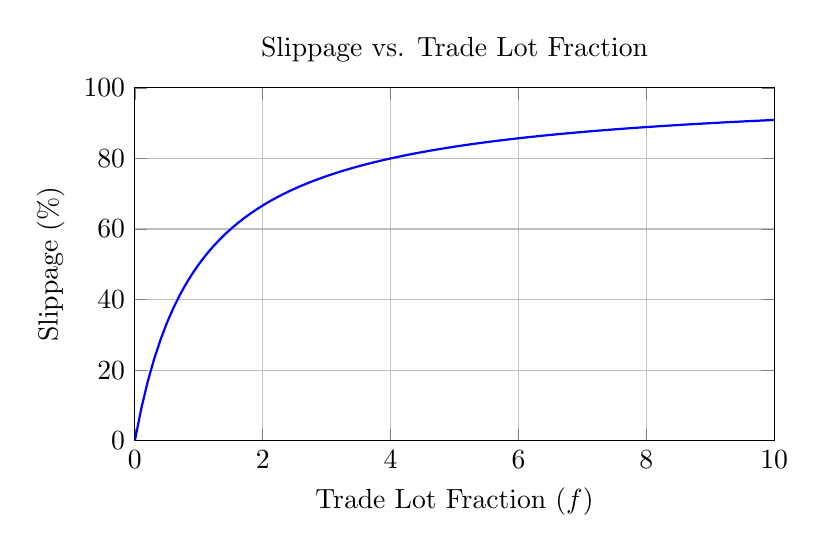
\begin{tikzpicture}
        \begin{axis}[
            xlabel={Trade Lot Fraction ($f$)},
            ylabel={Slippage (\%)},
            xmin=0, xmax=10,
            ymin=0, ymax=100,
            grid=major,
            width=0.8\textwidth,
            height=0.5\textwidth,
            legend pos=north west,
            title={Slippage vs. Trade Lot Fraction}
        ]
        \addplot[
            domain=0:10,
            samples=100,
            thick,
            blue
        ]
        {100 * x / (1 + x)};
        \end{axis}
    \end{tikzpicture}
    \caption{Plot of Slippage (\%) vs. Trade Lot Fraction ($f = \Delta x / x$)}
    \label{fig:slippage_fraction}
\end{figure}
\end{document}